\chapter{Desarrollo}

El presente capítulo está orientado a presentar la implementación de la metodología de desarrollo.

\section{Diseño de software }

A continuación, se presentan elementos claves en el diseño de software, tales como arquitecturas, modelos de datos y mockups.

\subsection{Arquitectura física }

La arquitectura física implementada corresponde a un modelo cliente-servidor. Durante la fase de desarrollo y pruebas, todos los componentes del sistema se alojan en un entorno local, utilizando contenedores Docker, lo que garantiza la portabilidad del entorno y elimina dependencias de configuración entre máquinas.

Como se ilustra en la Figura \ref{fig:arqfisica}, el flujo de comunicación comienza cuando el dispositivo cliente realiza una petición a través de Internet hacia el servidor de Frontend, donde se sirve la aplicación React. Las interacciones dinámicas del usuario generan peticiones HTTP/HTTPS hacia el servidor Backend desarrollado en Node.js, el cual se comunica con dos servicios externos: el Servidor de Base de Datos PostgreSQL, encargado de la persistencia de datos, y la API de Mensajería de WhatsApp, responsable del envío de recordatorios automáticos a los clientes.

Esta separación en contenedores independientes facilita una eventual migración hacia servicios en la nube especializados.

\begin{figure}[H]
  \centering
  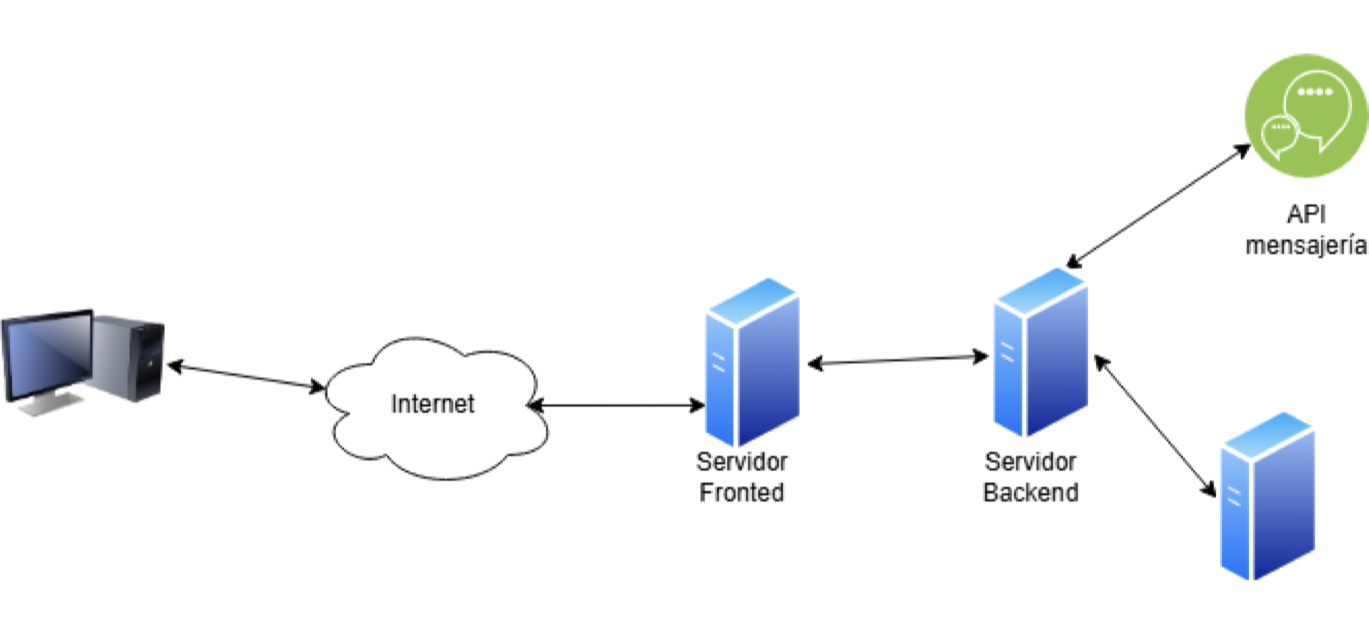
\includegraphics[width=0.8\textwidth]{fig-4-1-arquitectura-fisica}
  \caption[Arquitectura Física]{Arquitectura Física del Sistema.}
  \label{fig:arqfisica}
\vspace{-5.72pt}
\end{figure}

\subsection{Arquitectura lógica}

La arquitectura lógica propuesta sigue el patrón de tres capas.

\begin{figure}[h]
  \centering
  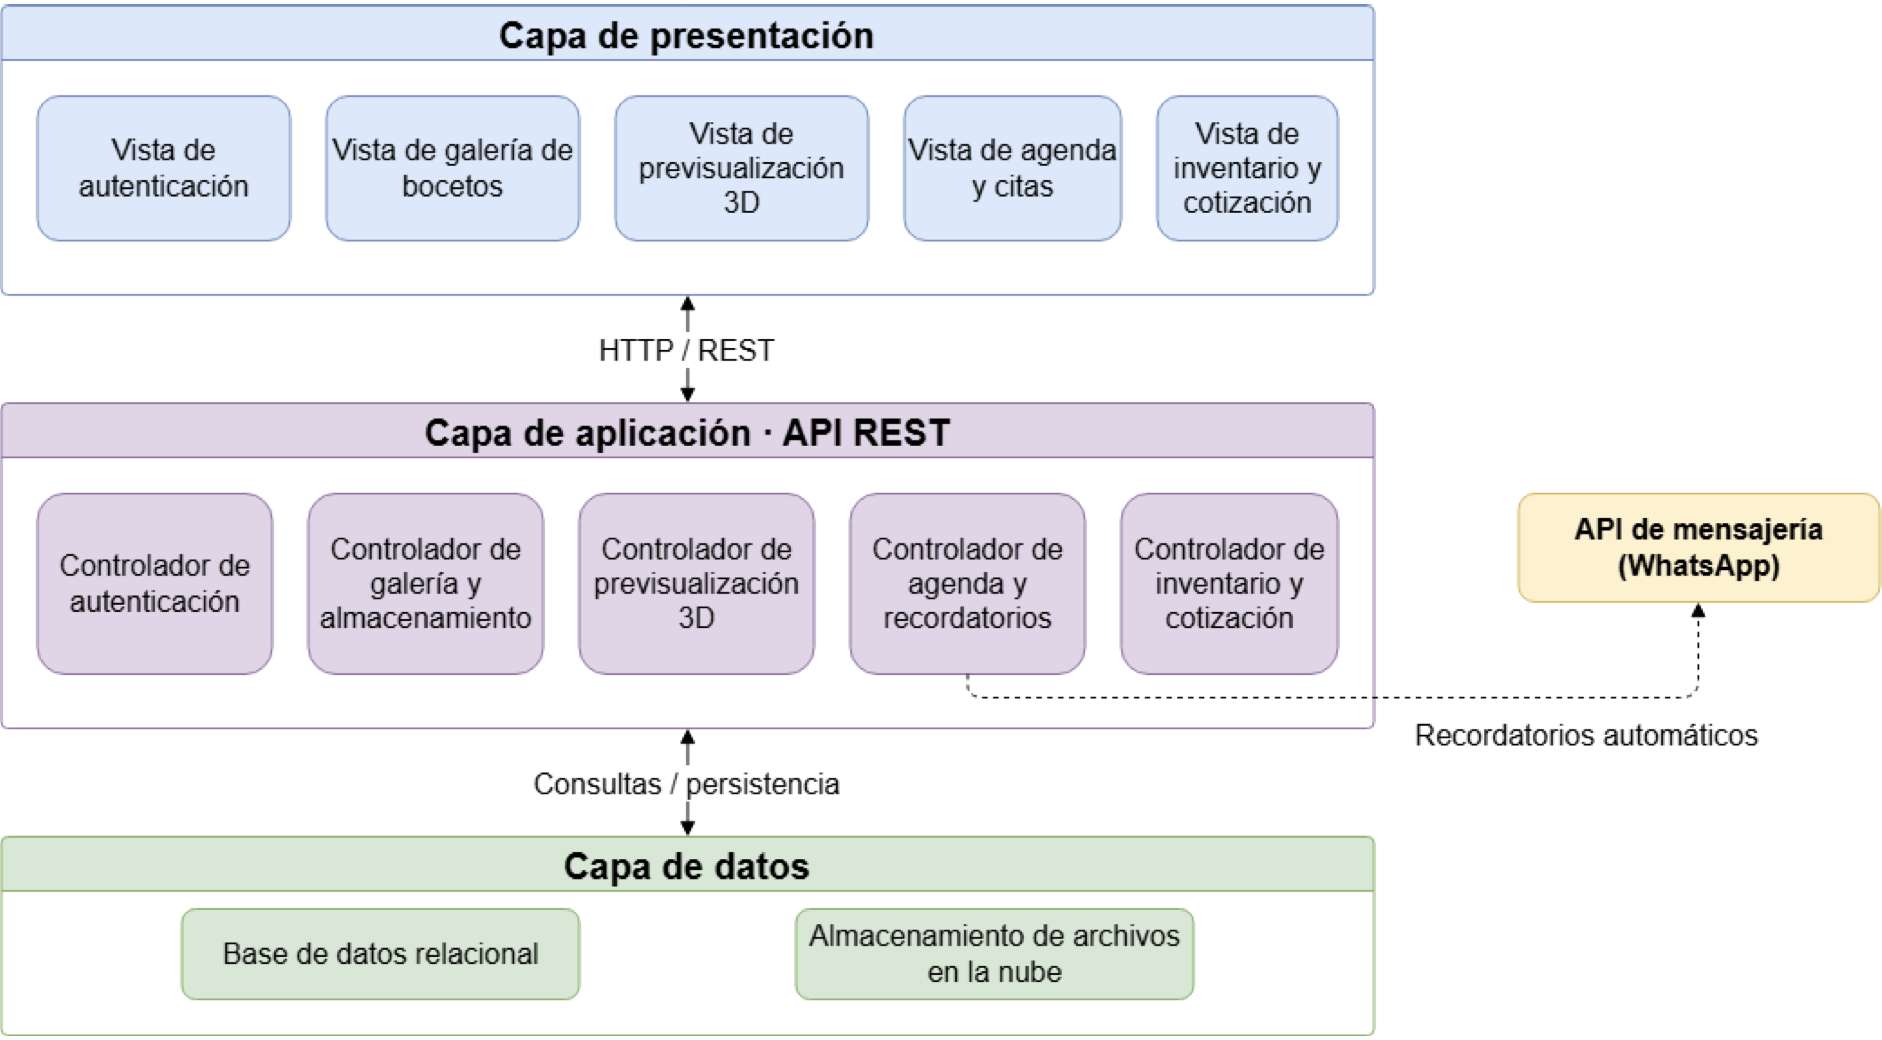
\includegraphics[width=1.1\textwidth]{fig-4-2-arquitectura-logica}
  \caption[Arquitectura Lógica]{Arquitectura Lógica del Sistema.}
  \label{fig:arqlogica}
\vspace{2.28pt}
\end{figure}

En la Figura \ref{fig:arqlogica} se ilustra la arquitectura lógica propuesta sigue el patrón de tres capas, ampliamente utilizado en el desarrollo de aplicaciones web modernas. Este patrón organiza el sistema en niveles de responsabilidad bien definidos, donde cada capa solo se comunica con la capa inmediatamente adyacente, lo que favorece la separación de responsabilidades, la mantenibilidad del código y la escalabilidad del sistema.

La capa de presentación corresponde a la interfaz de usuario ejecutada en el navegador del cliente. Esta capa es responsable de renderizar las vistas y gestionar la interacción del usuario, organizándose en módulos que corresponden a las funcionalidades principales del sistema: autenticación, galería de bocetos, previsualización 3D, agenda de citas, e inventario y cotización.

La capa de aplicación centraliza la lógica de negocio del sistema, expuesta mediante una API REST que recibe las solicitudes HTTP provenientes de la capa de presentación. Esta capa contiene los controladores de cada módulo, encargados de validar los datos de entrada, ejecutar las reglas de negocio como el algoritmo de cotización automática o el envío de recordatorios y coordinar las operaciones sobre la capa de datos.

La capa de datos es responsable de la persistencia del sistema. Se divide en dos componentes: la base de datos relacional, que almacena de forma estructurada los registros de usuarios, citas, inventario y cotizaciones, y el almacenamiento de archivos en la nube, dedicado a los bocetos en formato de imagen y los modelos anatómicos tridimensionales.

Adicionalmente, la capa de aplicación se integra con un servicio externo de mensajería para el envío automatizado de recordatorios a los clientes, manteniéndose esta integración desacoplada del resto del sistema mediante su propio controlador.

\subsection{Modelo de datos }

Como se mencionó en el Capítulo 2.3.3, el modelo de datos se basa en una base de datos relacional, utilizando PostgreSQL. A continuación, la Figura \ref{fig:er} muestra el diagrama entidad-relación del modelo de datos propuesto para el sistema.

\begin{figure}[H]
  \centering
  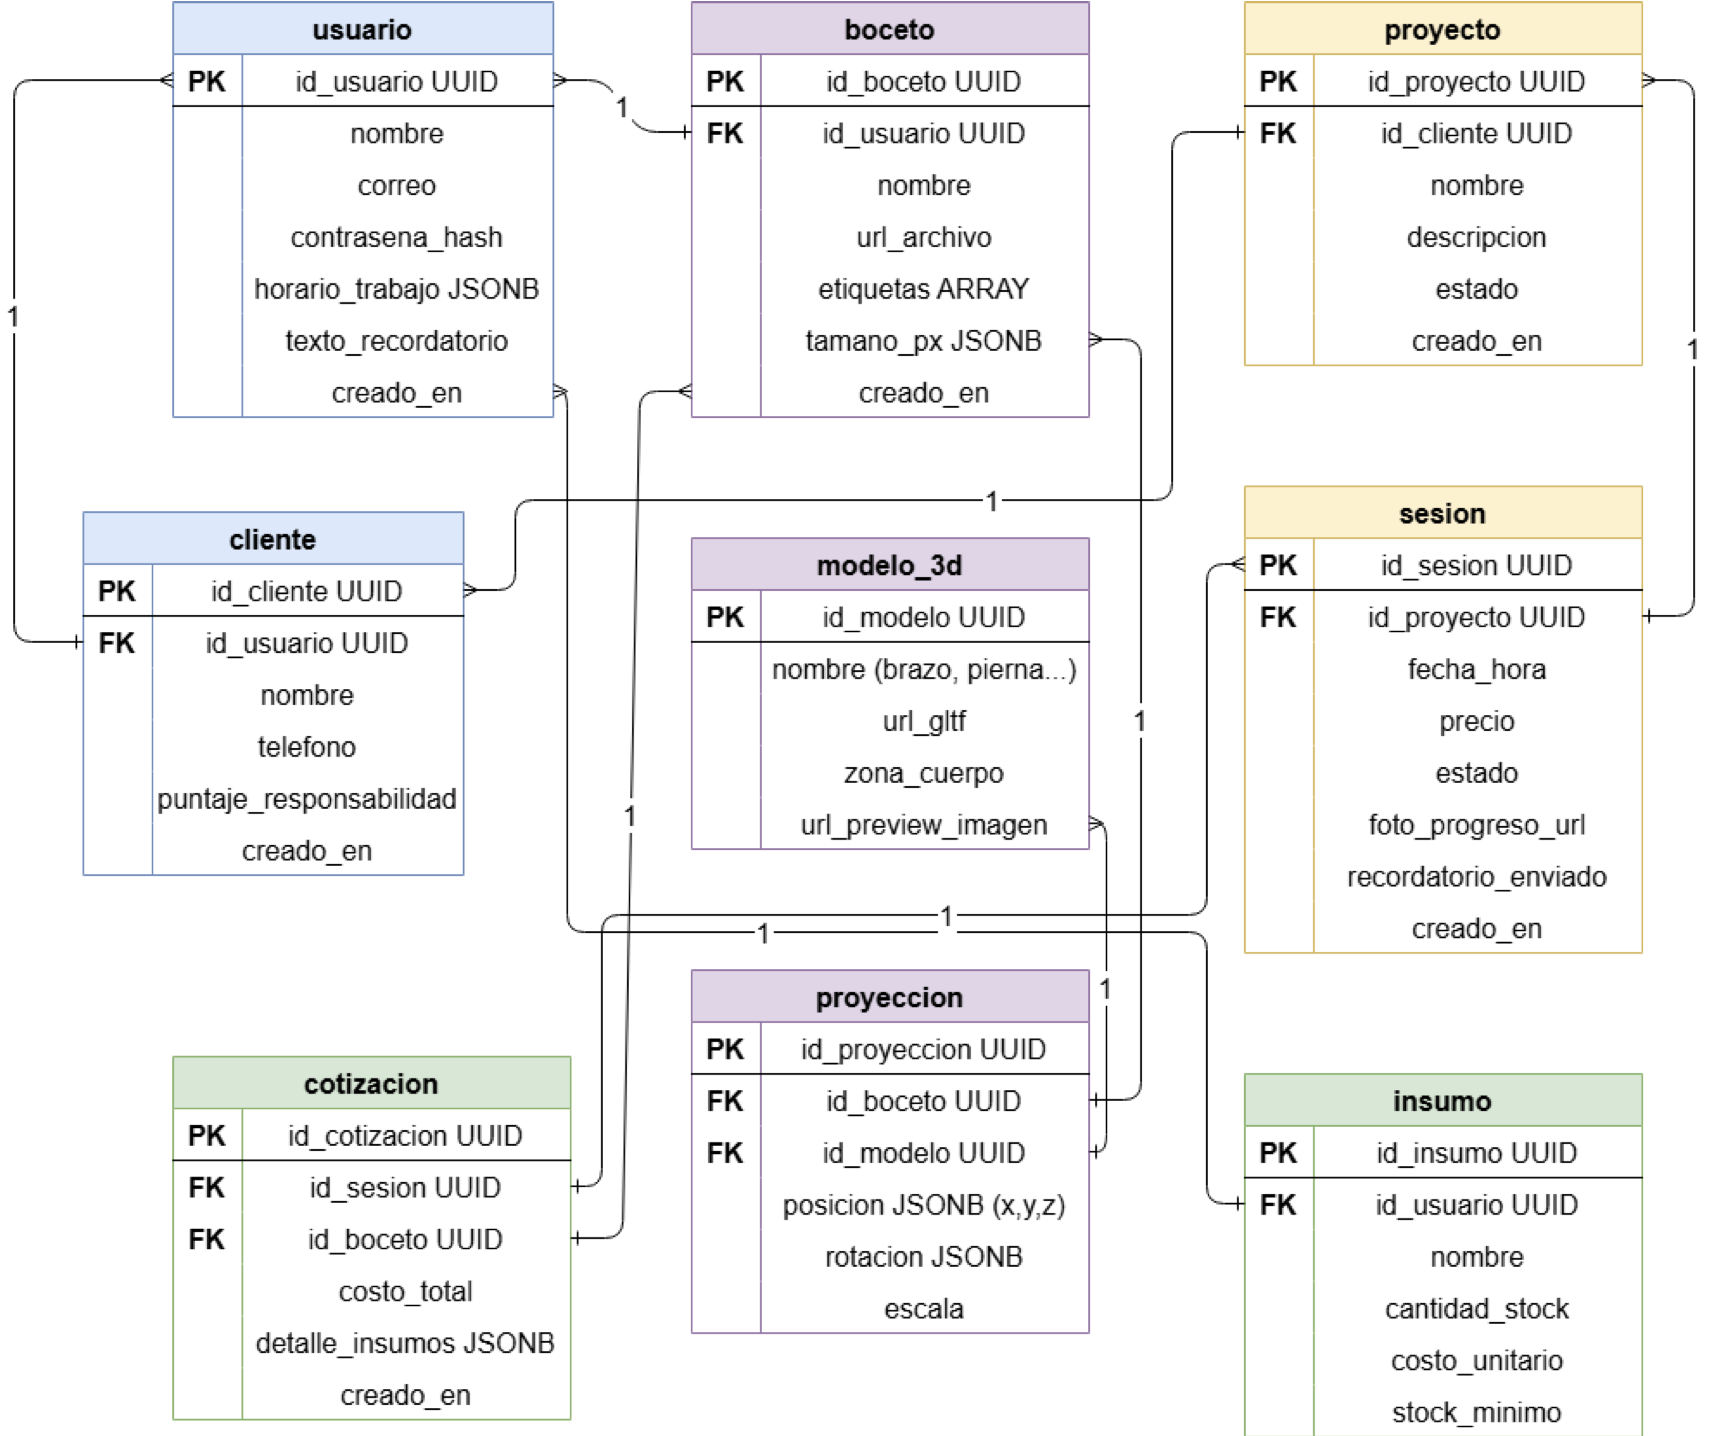
\includegraphics[width=\textwidth]{fig-4-3-diagrama-er}
  \caption[Diagrama Entidad-Relación]{Diagrama Entidad-Relación del modelo de datos del sistema.}
  \label{fig:er}
\end{figure}

\vspace{\parskip}
\subsection{Mockups}

En esta sección se presentan algunos de los mockups propuestos durante el proceso de desarrollo del sitema, los cuales fueron diseñados en base a los requerimientos funcionales y validos por la contrapartee. Estos mockups tienen como objetivo guiar el desarrollo de las principales interfaces del sistema y asegurando que cumplan con las expectativas del cliente experto.

\begin{figure}[H]
  \centering
  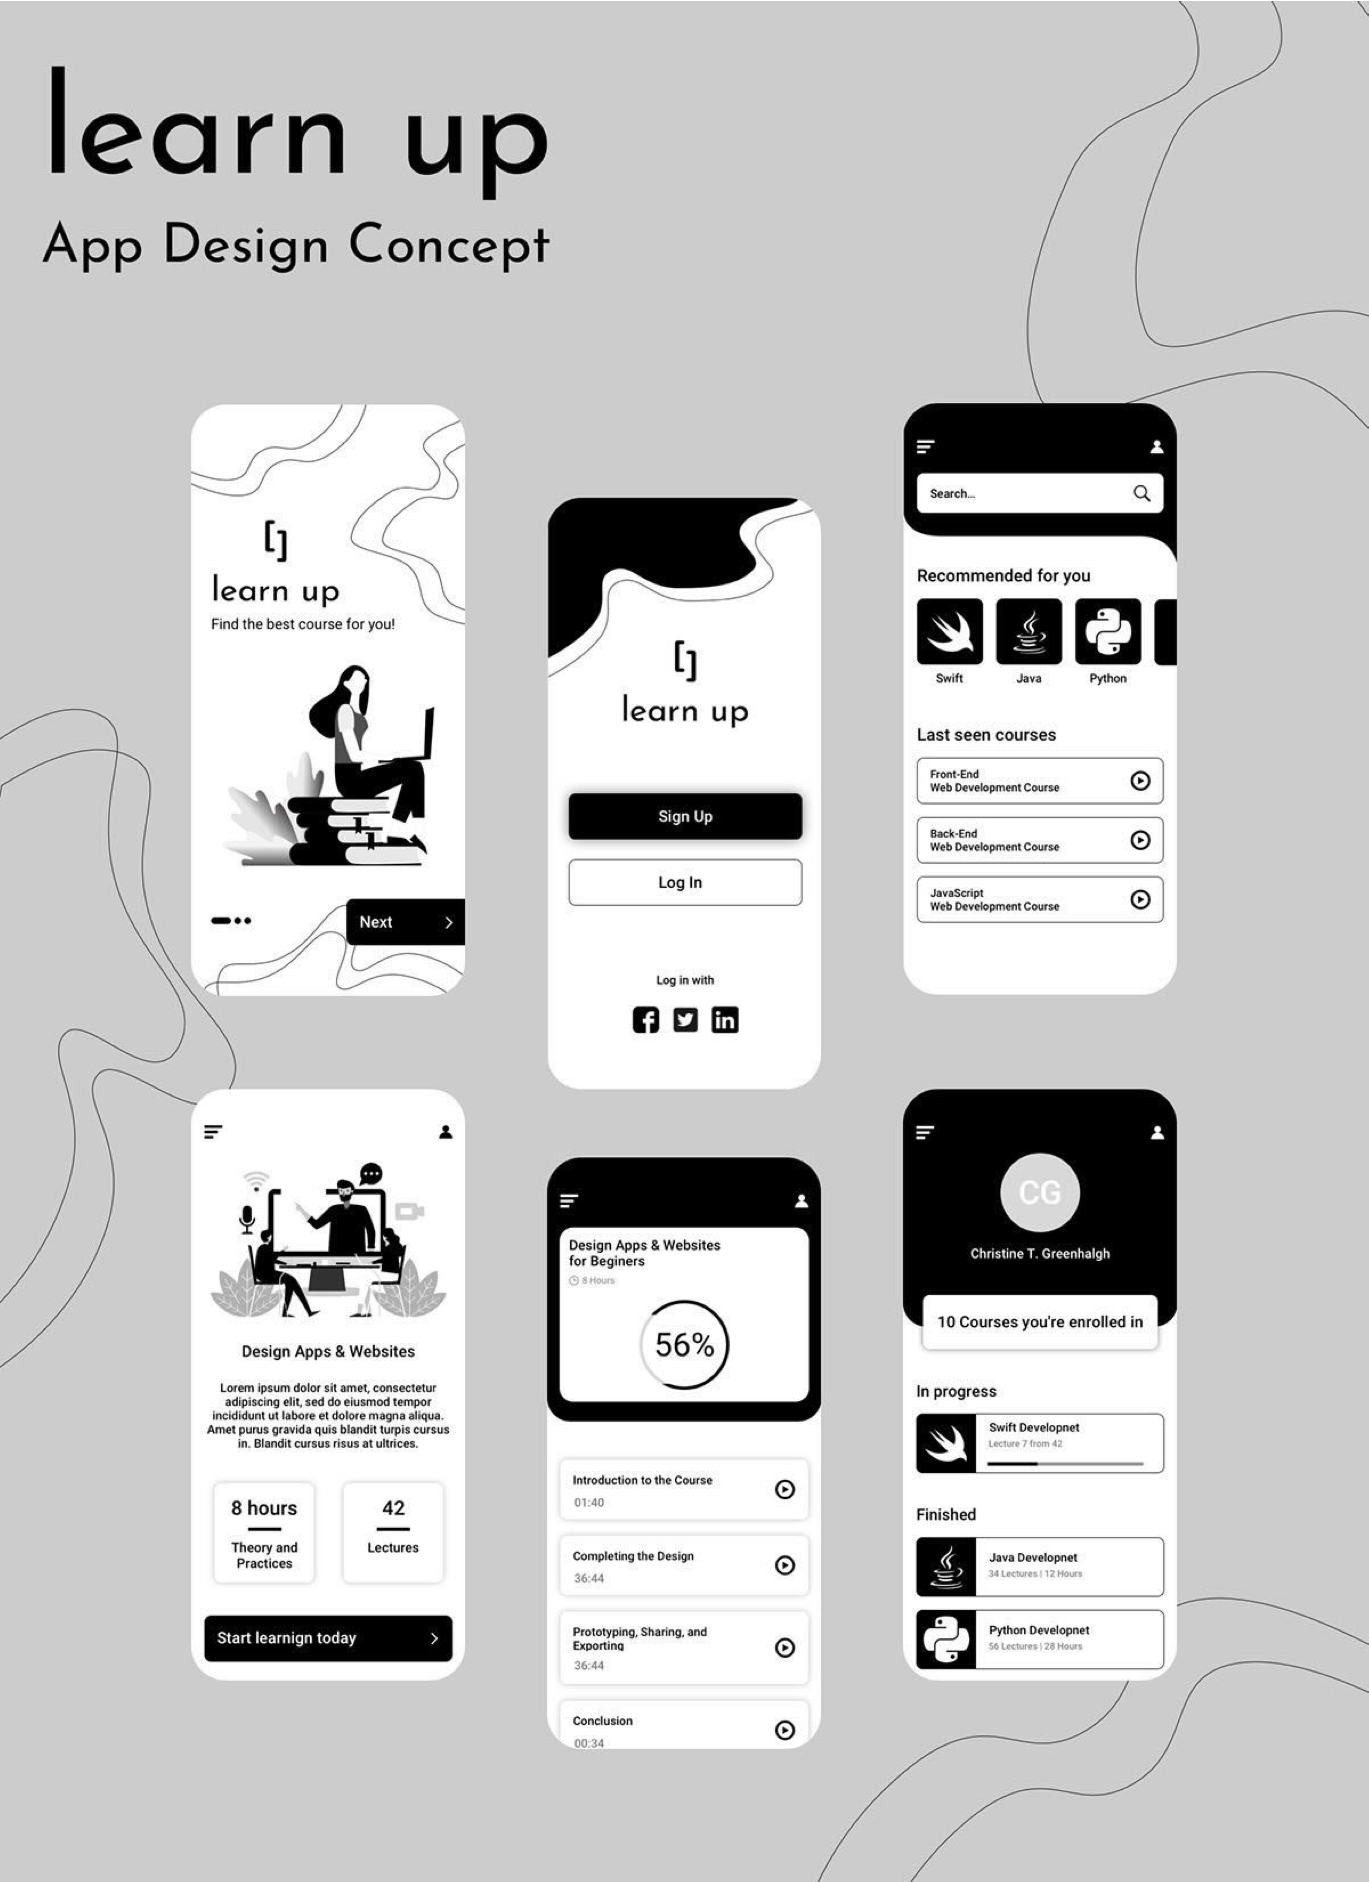
\includegraphics[width=0.8\textwidth]{fig-4-4-idea-1}
  \caption{Idea 1}
  \label{fig:idea1}
\end{figure}

\begin{figure}[H]
  \centering
  
\includegraphics[width=0.8\textwidth]{fig-4-5-idea-2}
  \caption{Idea 2}
  \label{fig:idea2}
\end{figure}

\begin{figure}[H]
  \centering
  
\includegraphics[width=0.8\textwidth]{fig-4-6-idea-3}
  \caption{Idea 3}
  \label{fig:idea3}
\end{figure}

En las Figuras \ref{fig:idea1}, \ref{fig:idea2} y \ref{fig:idea3} se presentan tres ideas de diseño para la interfaz de usuario del sistema, estas ideas fueron diseñadas por el usuario experto y buscan ser una guía visual para la elaboración de los mockups finales y la estética que se busca conseguir en la aplicación.

\begin{figure}[H]
  \centering
  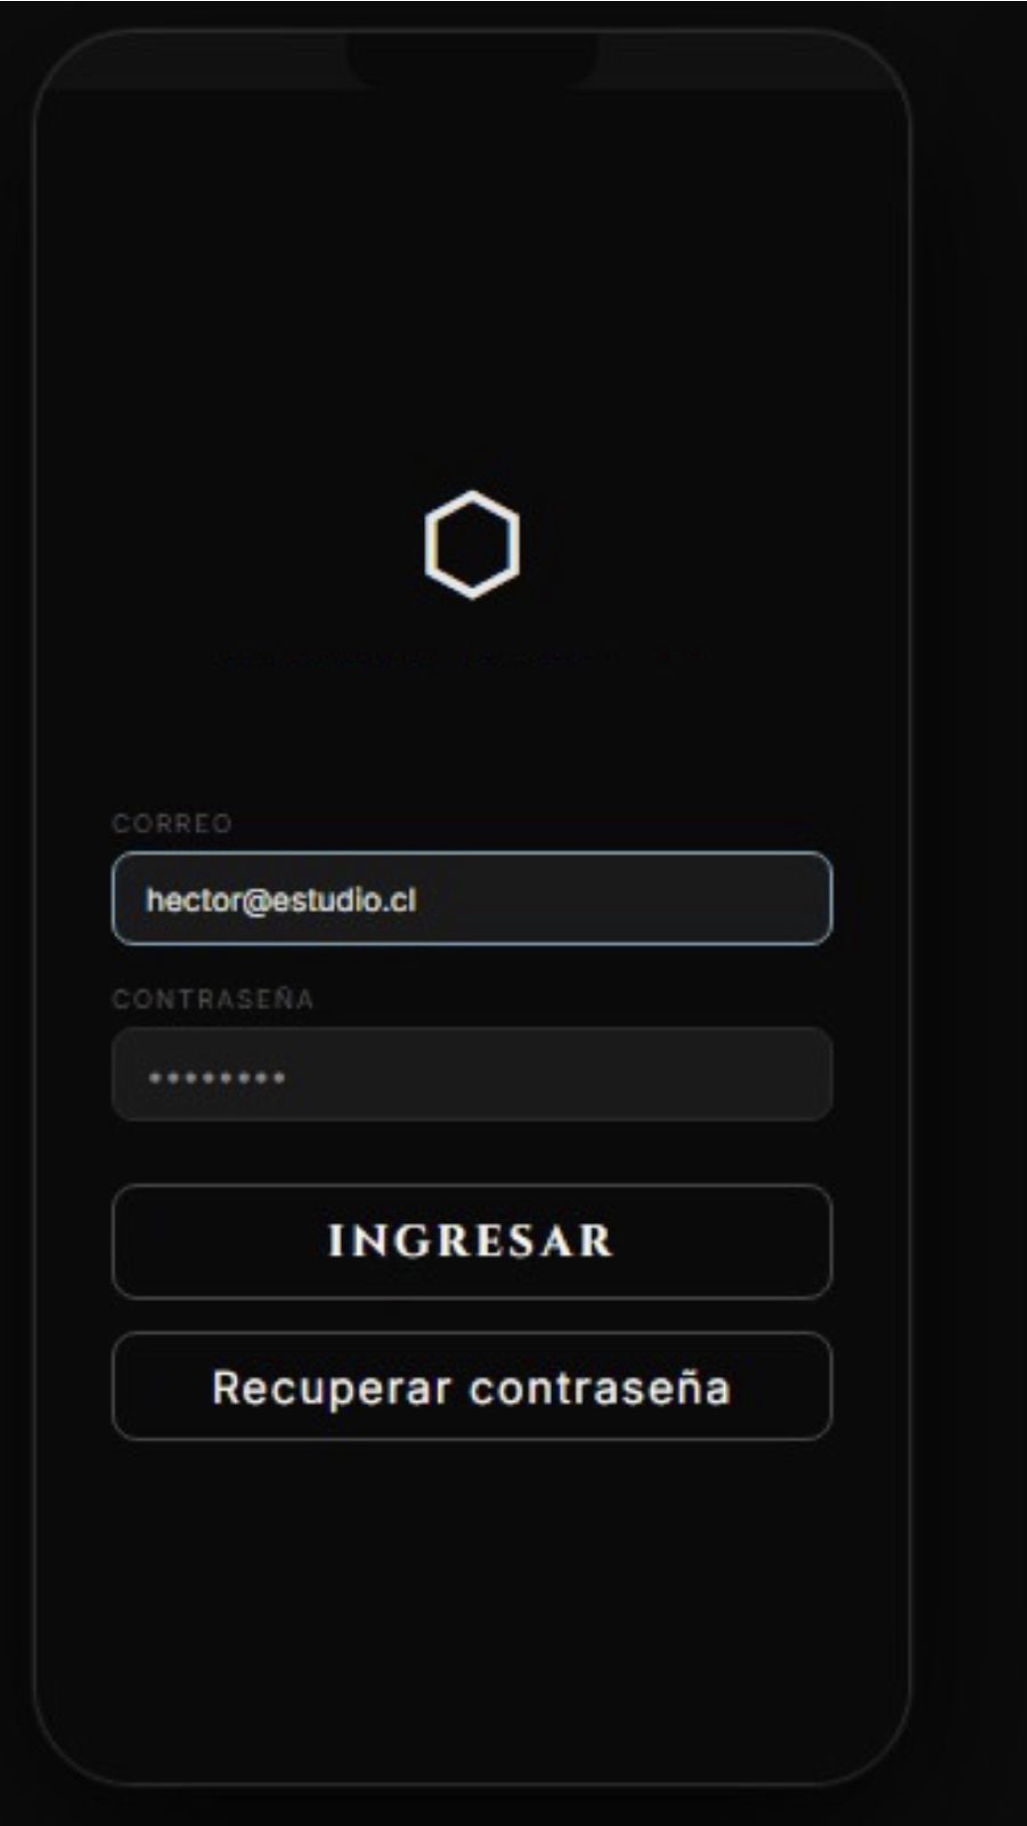
\includegraphics[width=0.6\textwidth]{fig-4-7-mockup-inicio-sesion}
  \caption[Mockup Inicio Sesión]{Mockup Inicio Sesión.}
  \label{fig:mockuplogin}
\end{figure}

La figura \ref{fig:mockuplogin} muestra la primera vista del usuario al ingresar a la aplicación, en el cual podrá iniciar sesión o redirigirse a la vista de ``Olvidé Mi Contraseña''.

\begin{figure}[H]
  \centering
  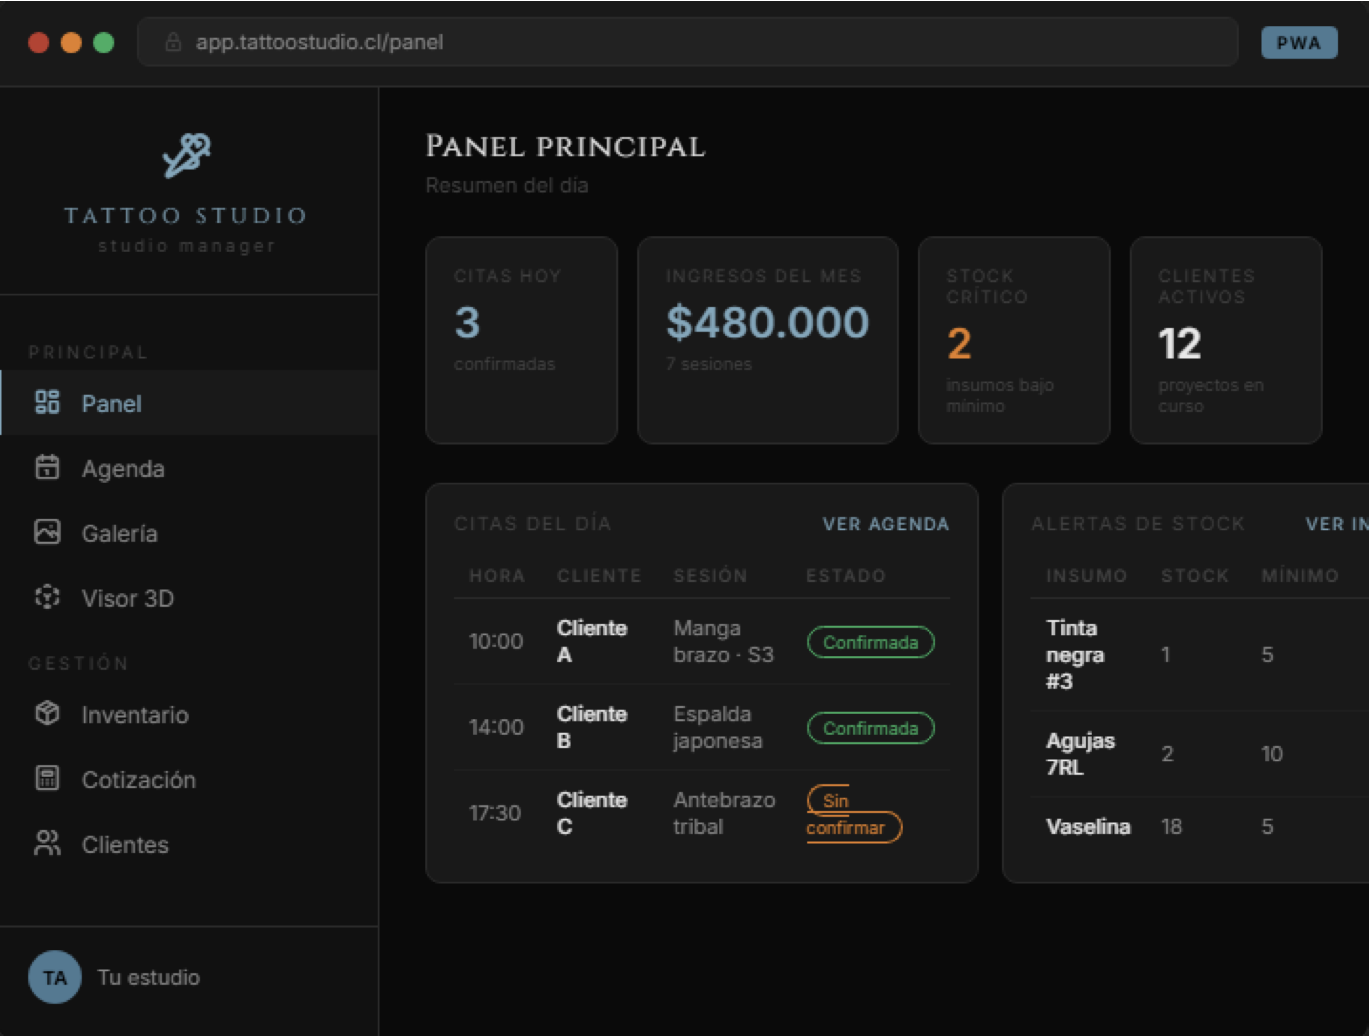
\includegraphics[width=0.8\textwidth]{fig-4-8-mockup-dashboard}
  \caption[Mockup Dashboard]{Mockup Dashboard.}
  \label{fig:mockupdashboard}
\end{figure}

\begin{figure}[H]
  \centering
  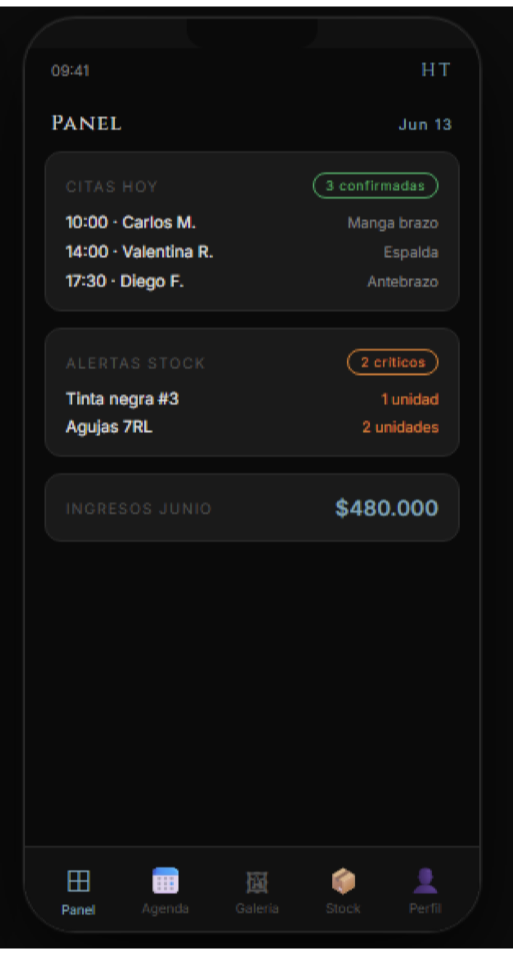
\includegraphics[width=0.3\textwidth]{fig-4-9-mockup-dashboard-movil}
  \caption[Mockup Dashboard Móvil]{Mockup Dashboard Móvil.}
  \label{fig:mockupdashboardmovil}
\end{figure}

La Figura \ref{fig:mockupdashboard} y \ref{fig:mockupdashboardmovil} muestran el diseño propuesto para el dashboard del sistema, tanto web como móvil, en el cual se muestran todos los componentes principales con lo que puede interactuar el usuario.

\begin{figure}[H]
  \centering
  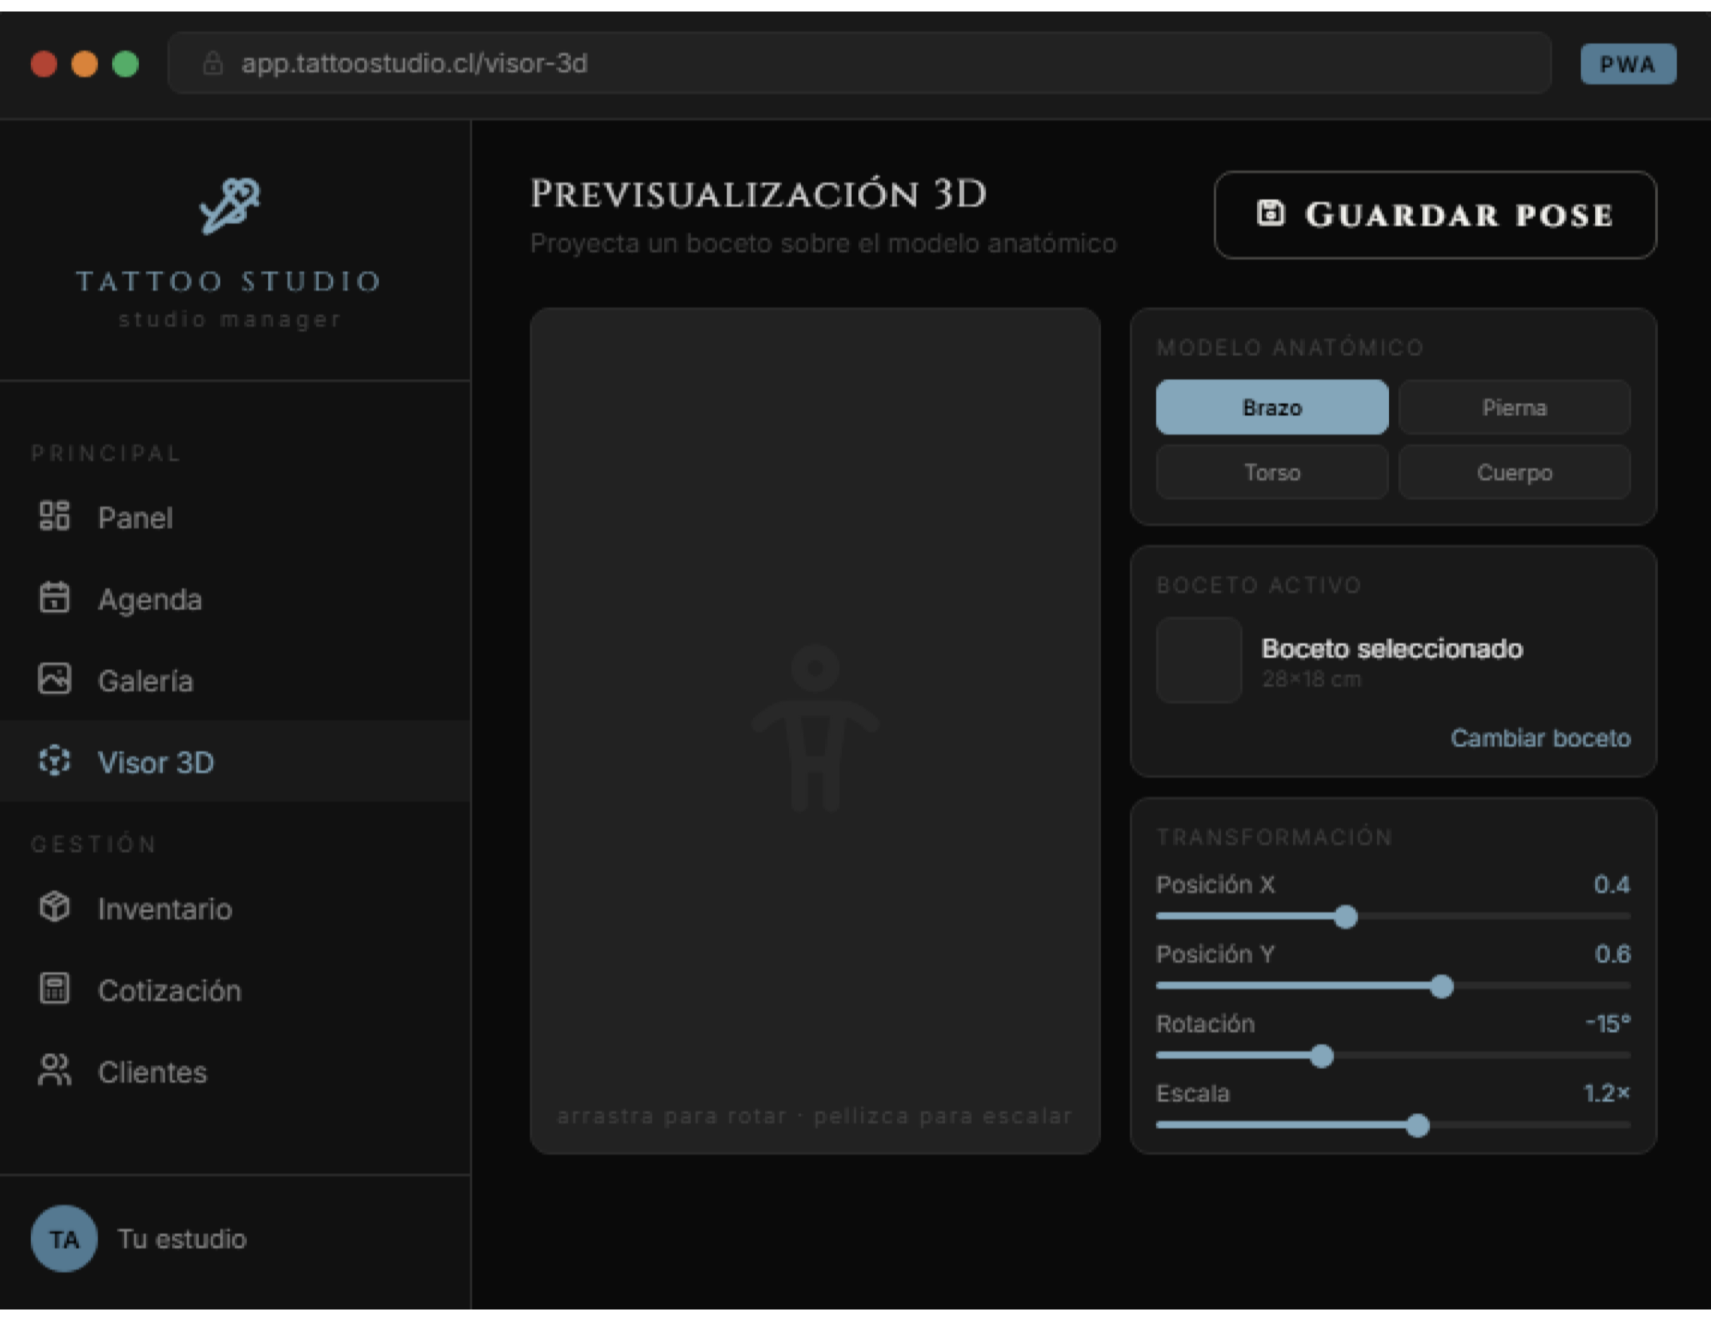
\includegraphics[width=\textwidth]{fig-4-10-mockup-previsualizacion-3d}
  \caption[Mockup Previsualización 3D]{Mockup Previsualización 3D.}
  \label{fig:mockup3d}
\end{figure}

\begin{figure}[H]
  \centering
  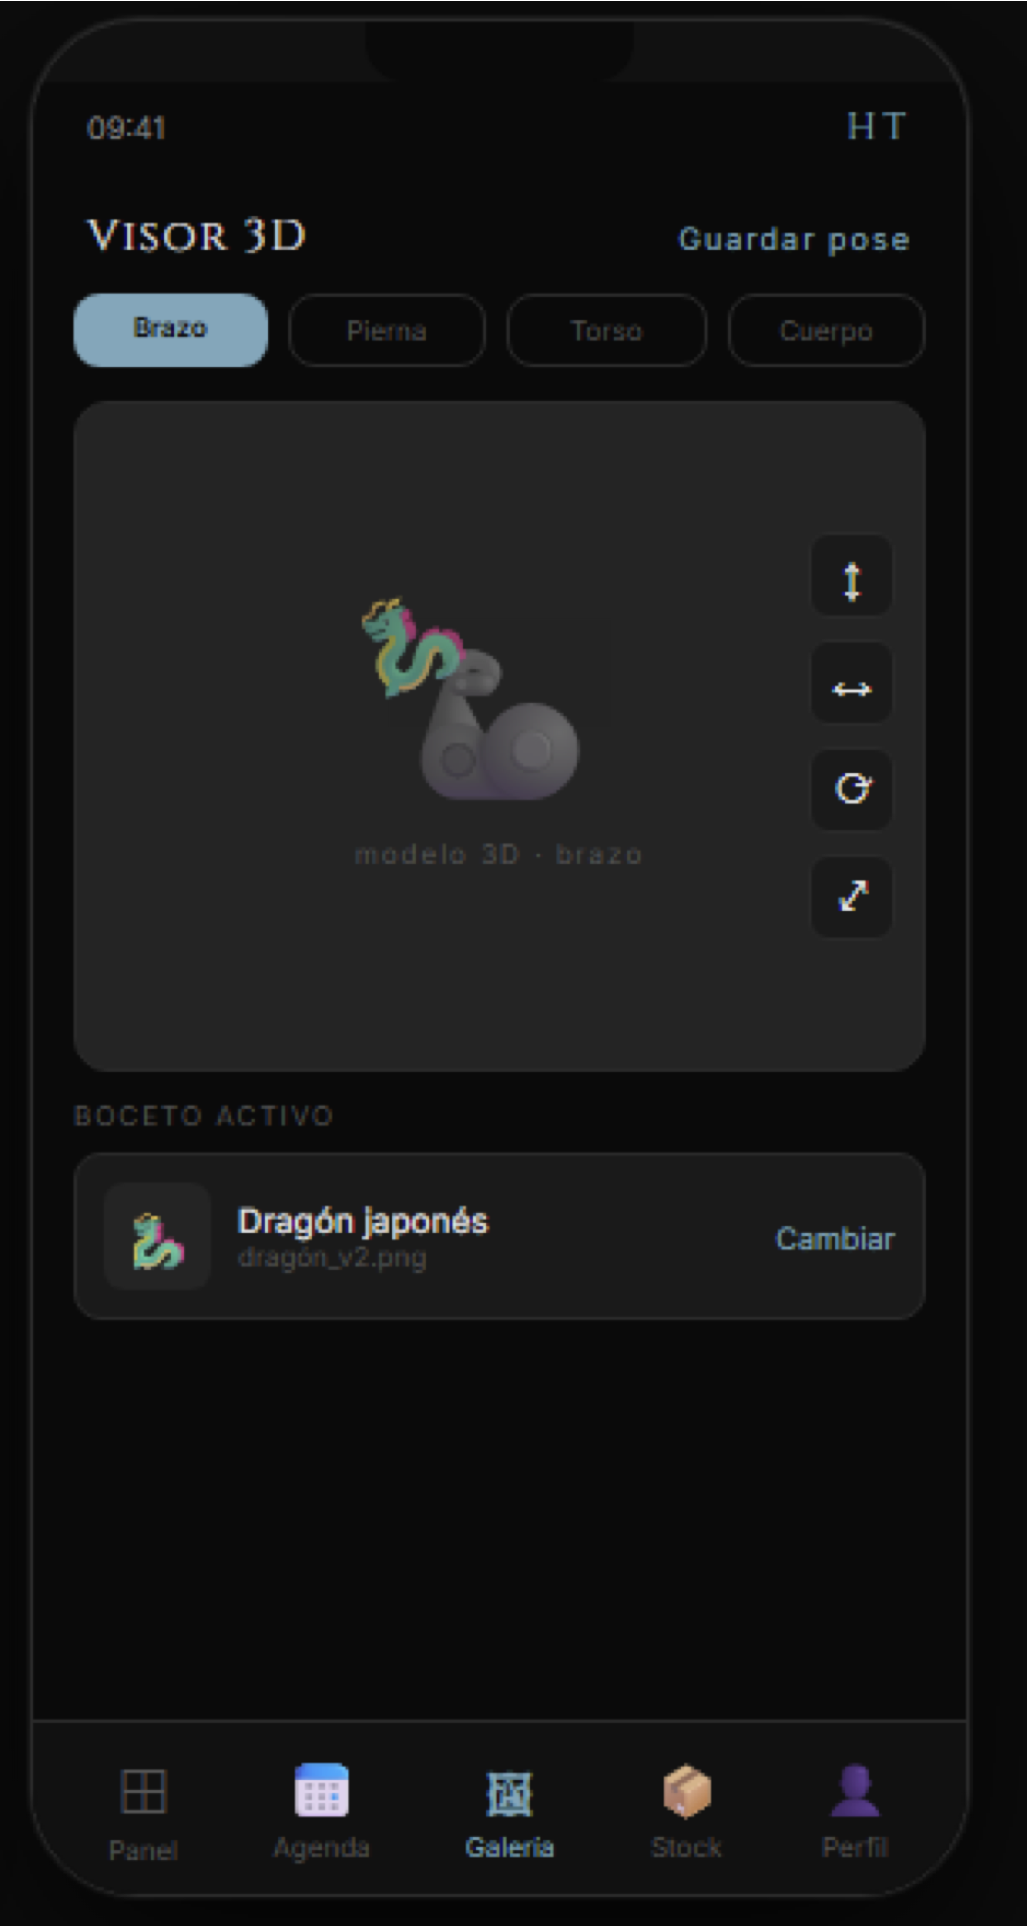
\includegraphics[width=0.6\textwidth]{fig-4-11-mockup-previsualizacion-3d-movil}
  \caption[Mockup Previsualización 3D Móvil]{Mockup Previsualización 3D Móvil.}
  \label{fig:mockup3dmovil}
\end{figure}

Por último, la Figura \ref{fig:mockup3d} y \ref{fig:mockup3dmovil} muestran el diseño propuesto para la vista de previsualización 3D, tanto web como móvil, en el cual se muestra la vista del modelo anatómico con el boceto proyectado sobre este, junto con las herramientas de ajuste para escalar, mover y rotar el diseño sobre el modelo 3D.

\section{Iteraciones}

A continuación, se detallan como se abordaron las iteraciones descritas en el Capítulo 3.1.2.

\subsection{Iteración 1}

En esta iteración, no existen historias de usuario asignadas, por lo que se enfocó en la planificación y diseño de la arquitectura del sistema, el modelo de datos y los mockups. Además, se establecieron las bases para el desarrollo de las siguientes iteraciones, definiendo los estándares de codificación, las herramientas a utilizar y la estructura general del proyecto.

\subsection{Iteración 2}

En esta iteración se comienza con la implementación de las historias de usuario HU01, HU02 y HU03, las cuales corresponden a la funcionalidad de autenticación. A continuación, se detalla la implementación siguiendo la metodología de desarrollo PXP.

\vspace{0.3cm}
\tituloparpegado{Inicio de Iteración}
En esta etapa, se crean y son registradas las tareas acordes a las historias de usuario, donde la Tabla \ref{tab:tareas} ilustra el registro de las tareas resultantes de la iteración.

\begin{table}[H]
  \centering
  \caption{Tareas asociadas a la Iteración 2}
  \label{tab:tareas}
  \renewcommand{\arraystretch}{1.2}
  \begin{tabular}{|l|l|p{8cm}|}
    \hline
    \textbf{Historia} & \textbf{Tarea} & \textbf{Descripción} \\
    \hline
    HU001 & T0001 & Crear diagrama de secuencia \\ \hline
    HU001 & T0002 & Crear ruta para inicio de sesión \\ \hline
    HU001 & T0003 & Crear vista para inicio de sesión \\ \hline
    HU002 & T0001 & Crear diagrama de secuencia \\ \hline
    HU002 & T0002 & Crear dashboard inicial \\ \hline
    HU002 & T0003 & Crear vista para cerrar sesión \\ \hline
    HU003 & T0001 & Crear diagrama de secuencia \\ \hline
    HU003 & T0002 & Crear ruta para olvidar contraseña \\ \hline
    HU003 & T0003 & Crear ruta para cambiar contraseña \\ \hline
    HU003 & T0004 & Crear vista para olvidar contraseña \\ \hline
    HU003 & T0005 & Crear vista para cambiar contraseña \\ \hline
    HU001, HU002, HU003 & T0009 & Creación y testeo de pruebas unitarias \\ \hline
    HU001, HU002, HU003 & T0010 & Creación y uso de sistema de pruebas \\ \hline
  \end{tabular}
\end{table}

\vspace{0.3cm}
\tituloparpegado{Diseño}
En esta etapa, se crean los diagramas de secuencia de las historias de usuario asociadas a la iteración. A continuación, las Figuras \ref{fig:seclogin}, \ref{fig:secdashboard} y \ref{fig:secolvido} ilustran el flujo de las principales funcioanlidades.

\begin{figure}[H]
  \centering
  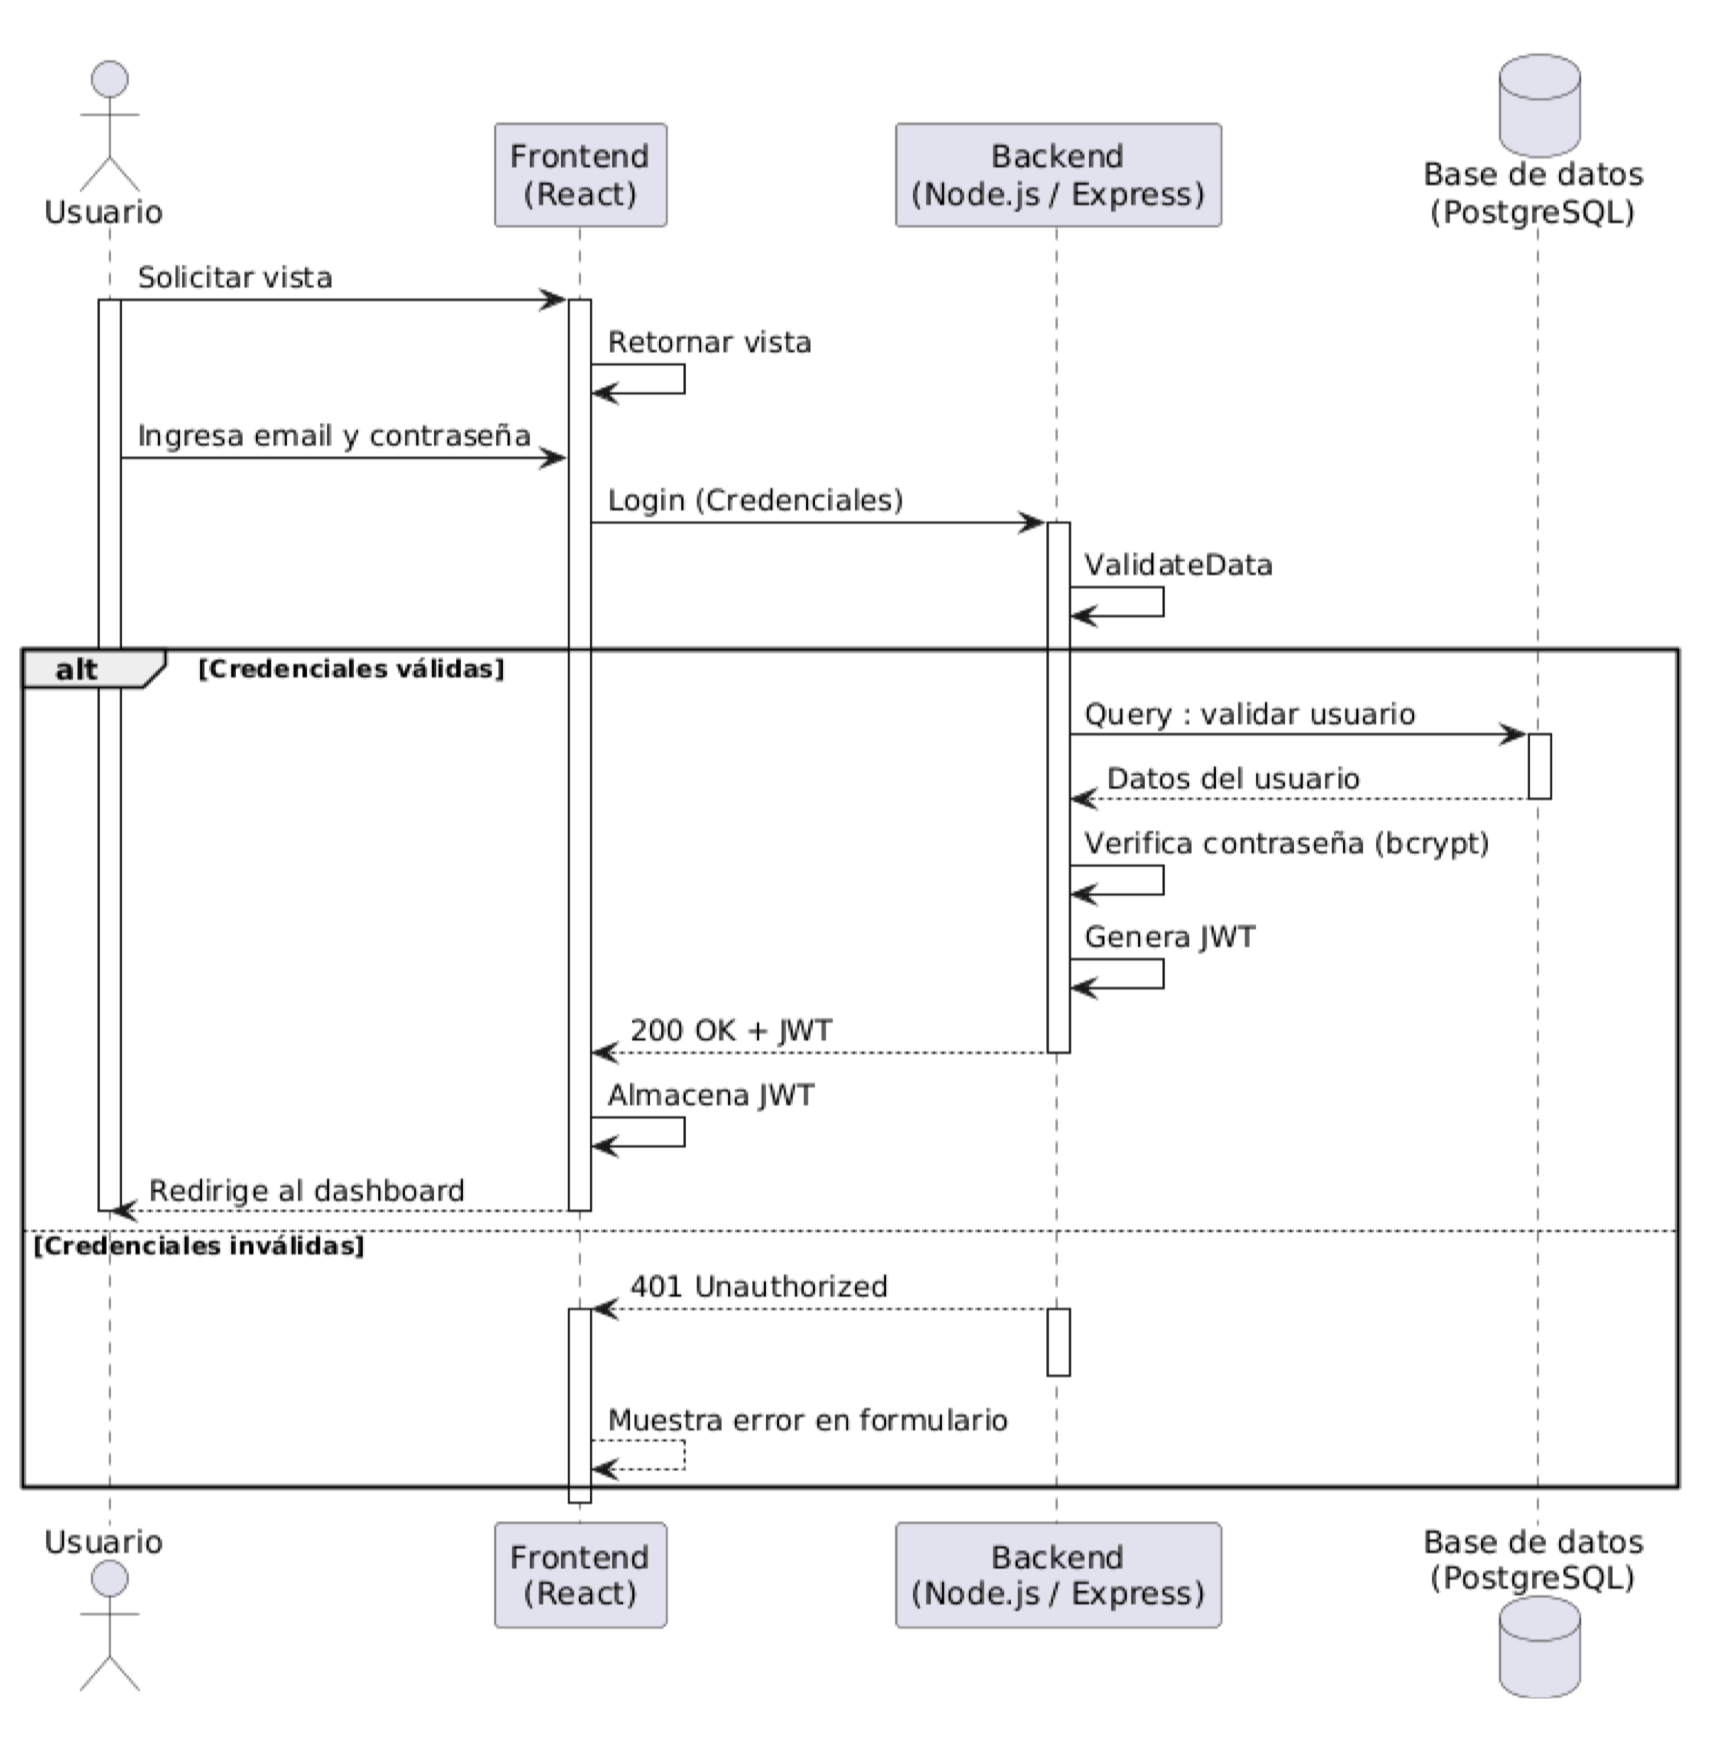
\includegraphics[width=\textwidth]{fig-4-12-secuencia-login}
  \caption[Diagrama de secuencia Inicio Sesión]{Diagrama de secuencia HU01: Login.}
  \label{fig:seclogin}
\end{figure}

\begin{figure}[H]
  \centering
  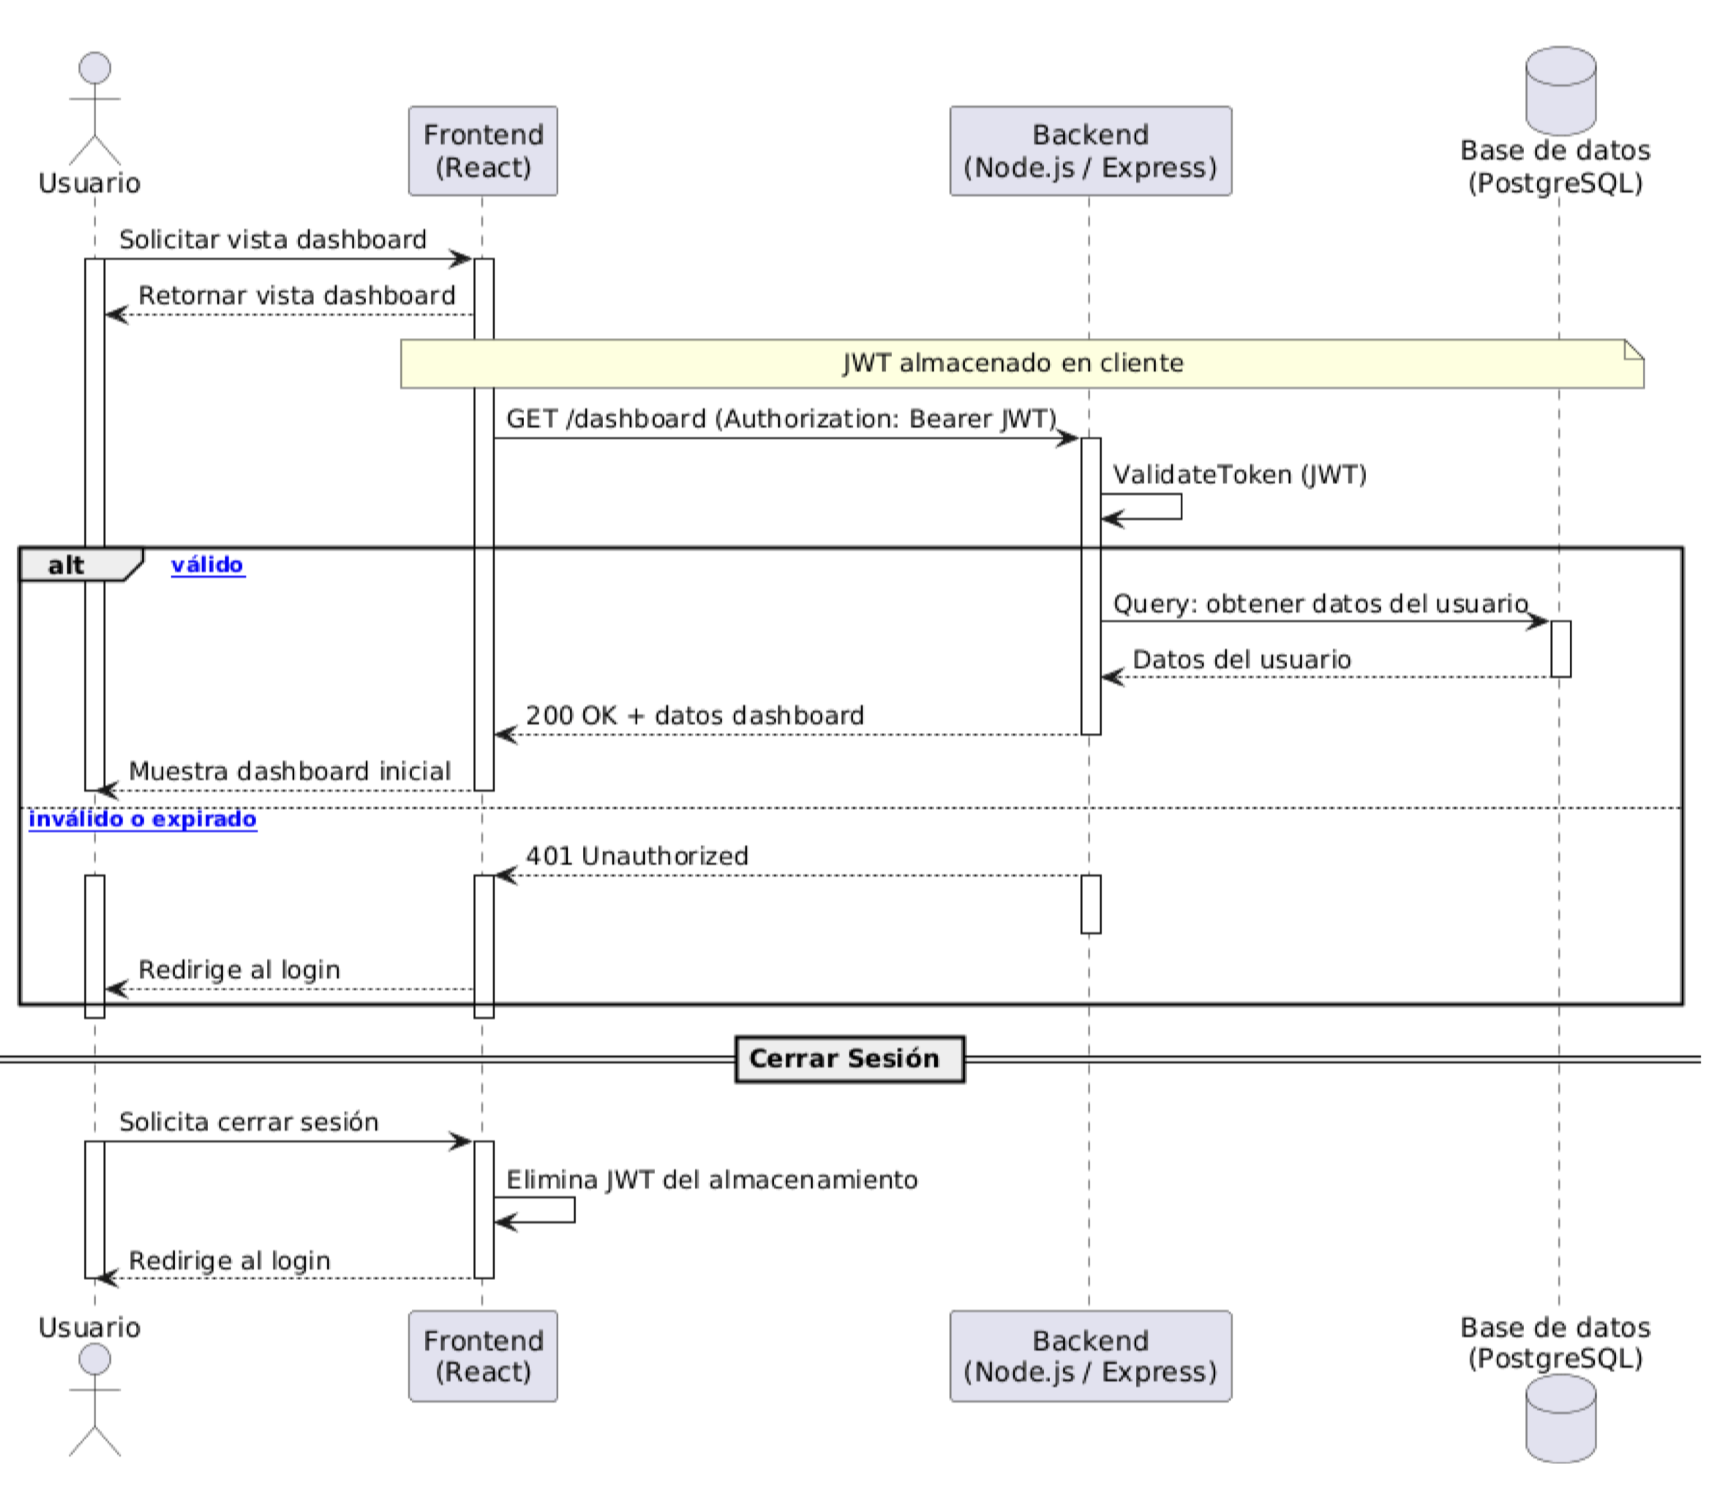
\includegraphics[width=\textwidth]{fig-4-13-secuencia-dashboard}
  \caption[Diagrama de secuencia Dashboard]{Diagrama de secuencia HU02: Dashboard.}
  \label{fig:secdashboard}
\end{figure}

\begin{figure}[H]
  \centering
  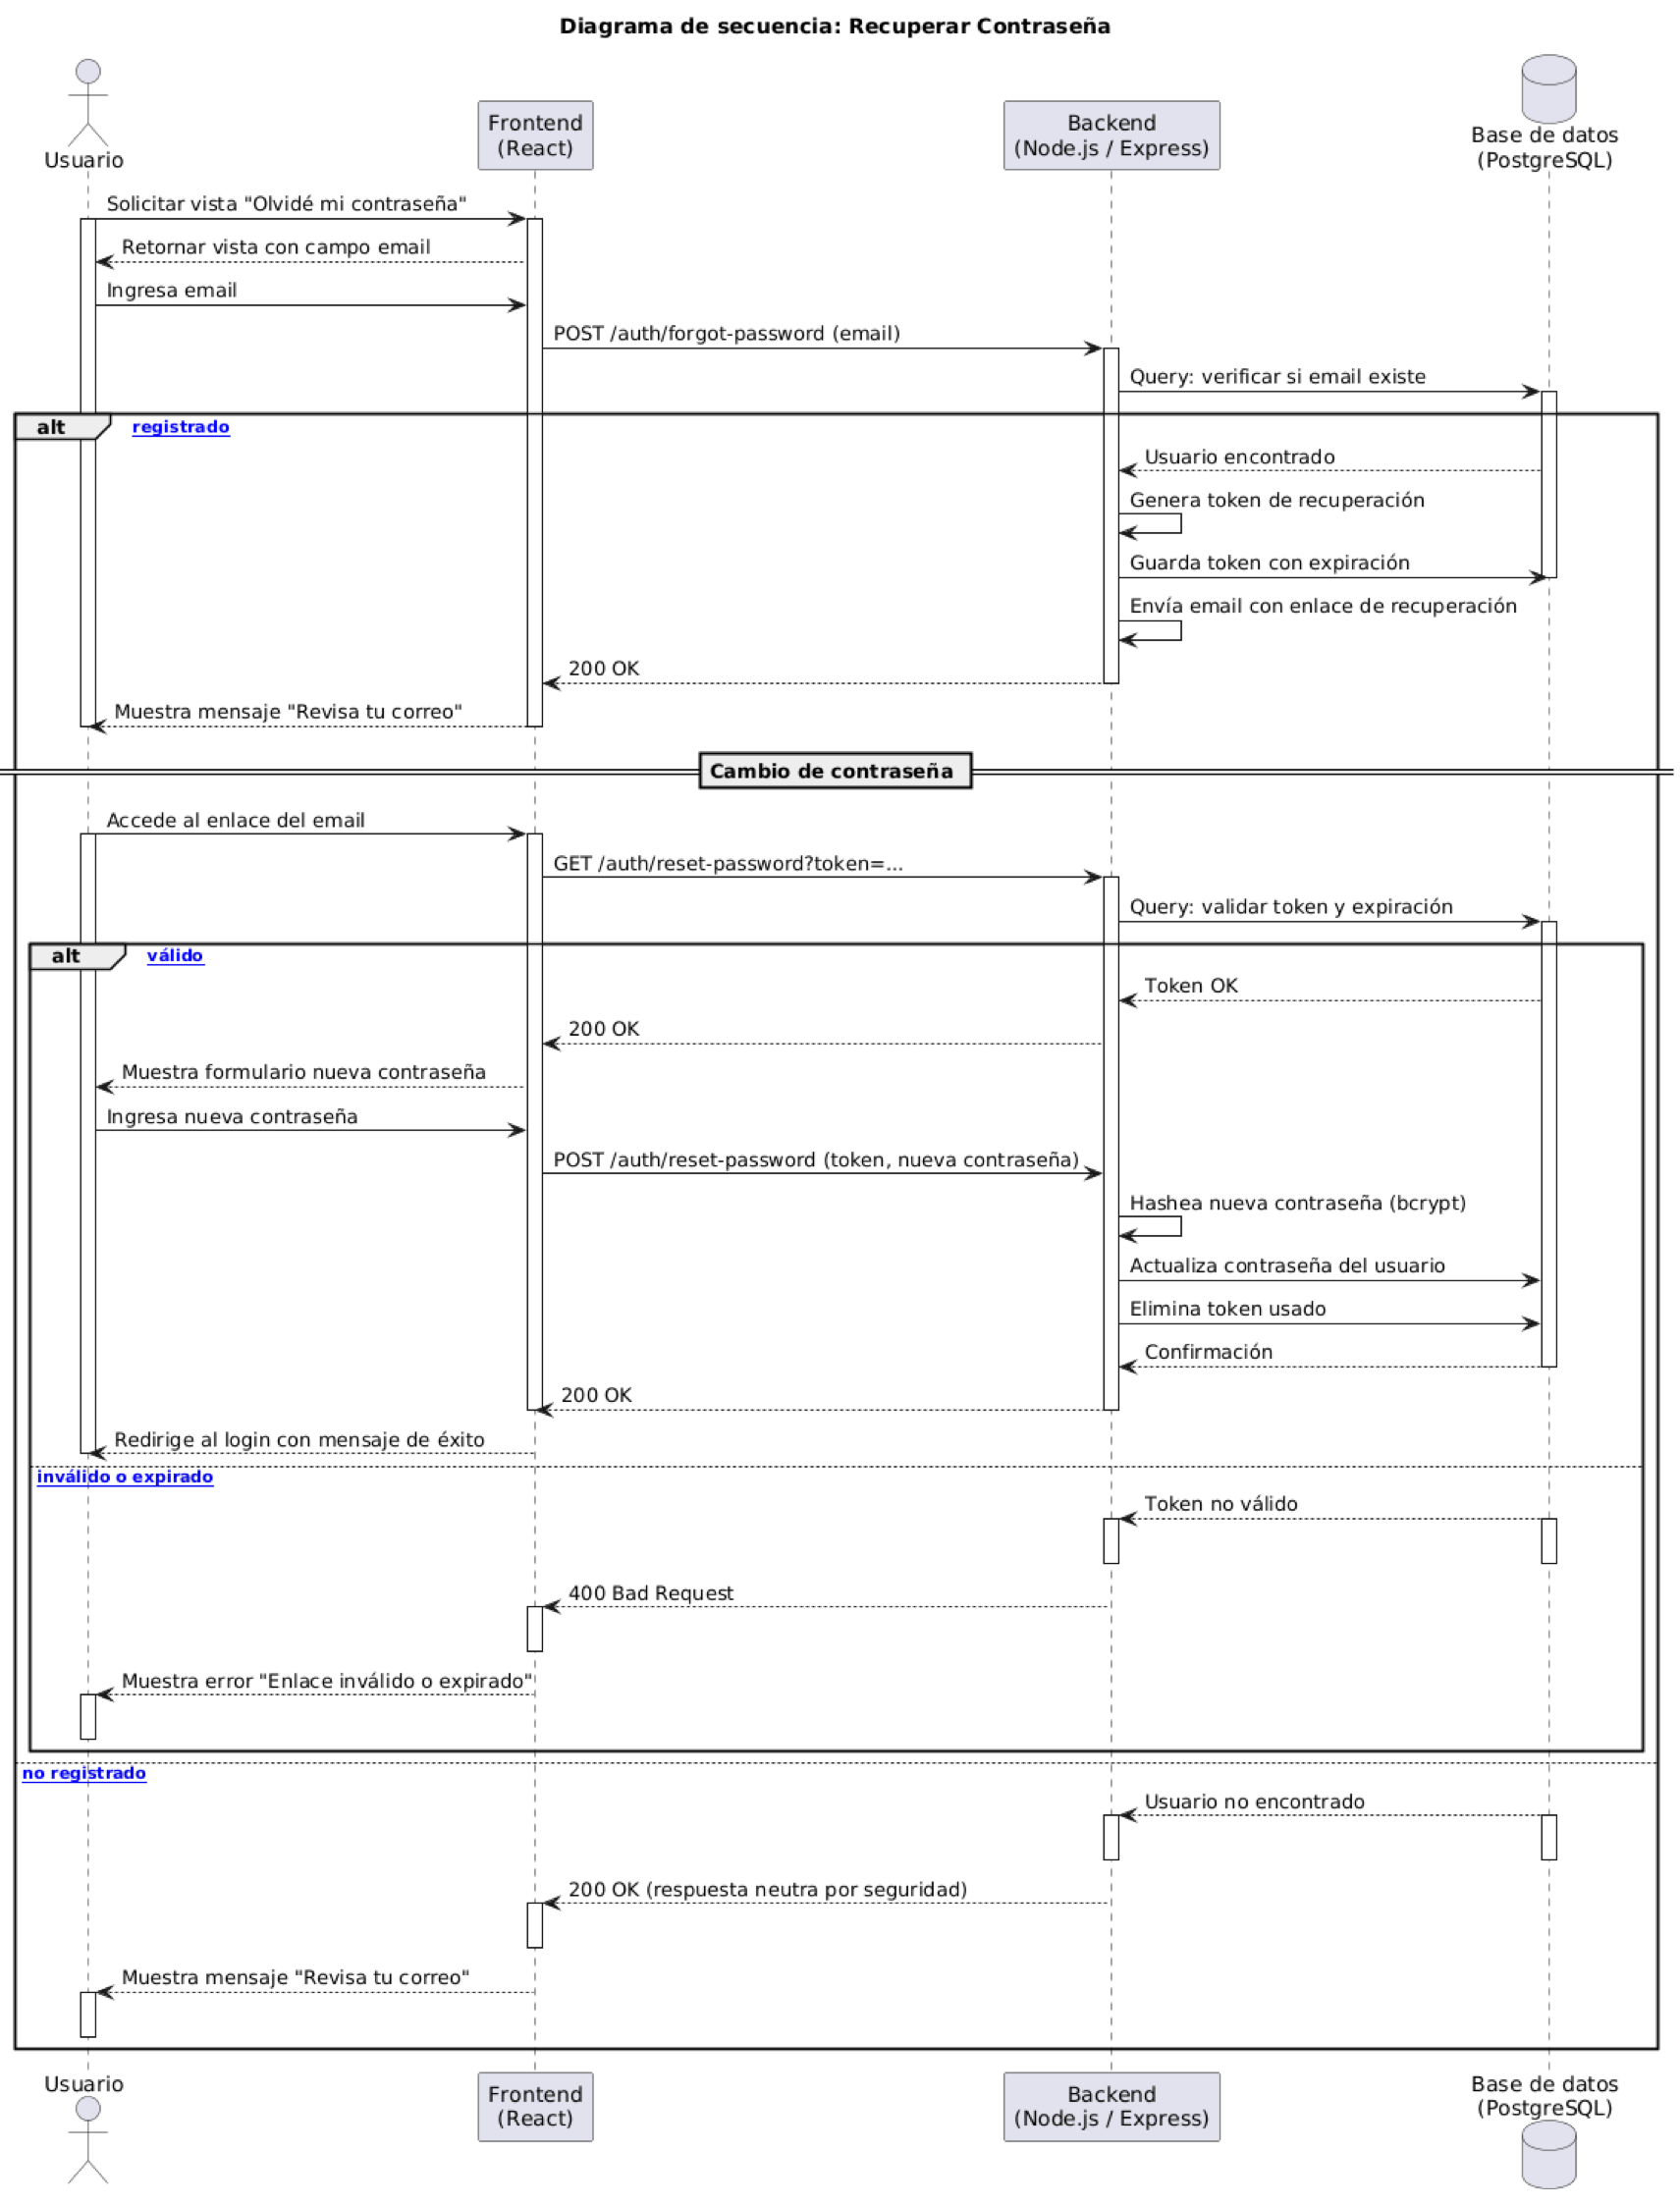
\includegraphics[width=\textwidth]{fig-4-14-secuencia-olvidar-contrasena}
  \caption[Diagrama de secuencia Olvidar Contraseña]{Diagrama de secuencia HU03: Olvidar Contraseña.}
  \label{fig:secolvido}
\end{figure}

\tituloparpegado{Implementación}
En esta etapa, se desarrolla tanto el backend como el frontend de las historias de usuario asignadas a la iteración. Se crean las rutas necesarias en el backend para manejar las solicitudes de inicio de sesión, cierre de sesión y recuperación de contraseña, mientras que en el frontend se desarrollan las vistas correspondientes para que el usuario pueda interactuar con estas funcionalidades. En el caso del inicio de sesión, se implemente JSON Web Tokens (JWT) para la autenticación y autorización de usuarios, asegurando acceso seguro a rutas protegidas del sistema. (Figura \ref{fig:jwt})

\begin{figure}[H]
  \centering
  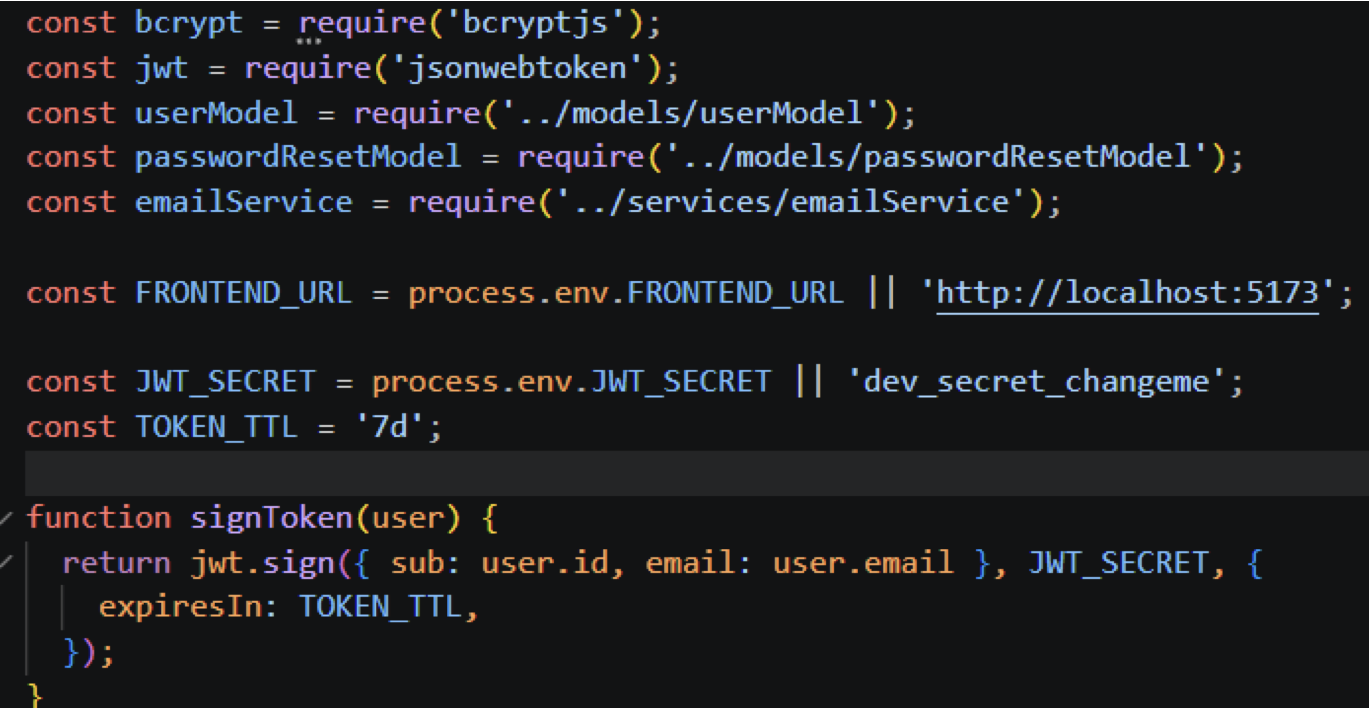
\includegraphics[width=0.8\textwidth]{fig-4-15-implementacion-jwt}
  \caption[Implementación JWT]{Implementación de autenticación mediante JSON Web Tokens (JWT).}
  \label{fig:jwt}
\end{figure}

Otro modulo que se implementó fue el servicio de envío de correos electrónicos para la funcionalidad de recuperación de contraseña, utilizando una librería de Node.js (Nodemailer) para enviar correos a través de un servicio SMTP, lo que permite a los usuarios recibir un enlace para restablecer su contraseña de manera segura como se puede ver en la Figura \ref{fig:email}.

\begin{figure}[H]
  \centering
  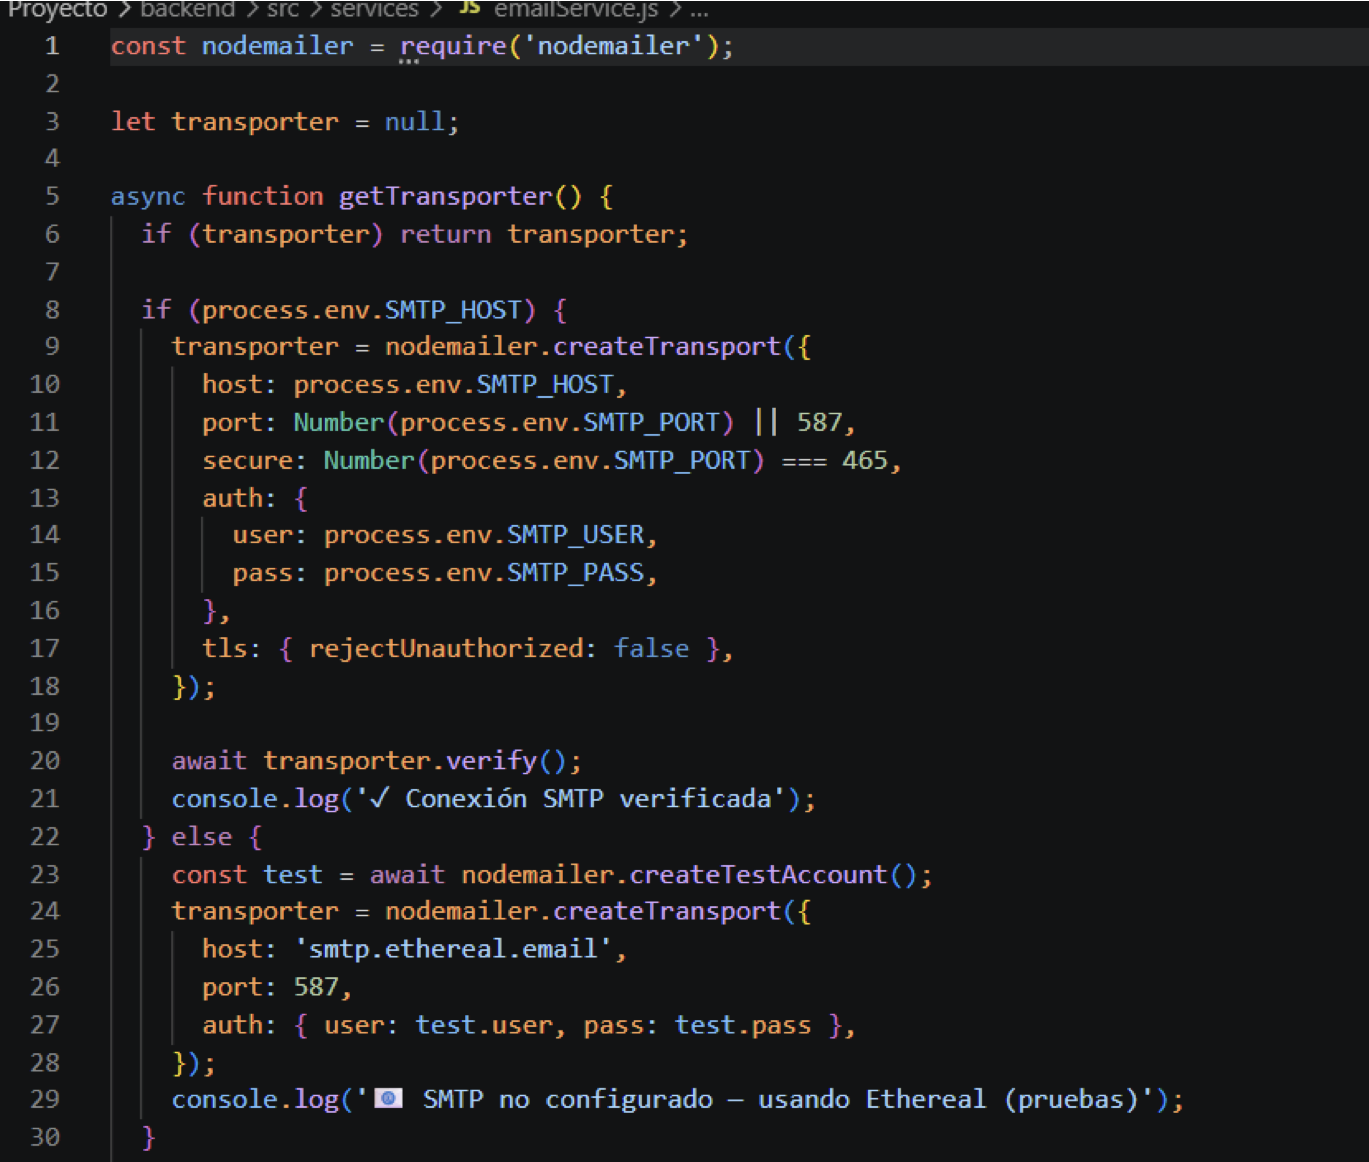
\includegraphics[width=0.8\textwidth]{fig-4-16-implementacion-email}
  \caption[Implementación Email]{Implementación del servicio de envío de correos electrónicos para recuperación de contraseña.}
  \label{fig:email}
\end{figure}

Al finalizar el desarrollo de las funcionalidades, se crean las pruebas unitarias correspondientes para cada una de las tareas definidas en el Inicio de Iteración, utilizando un framework de pruebas como Jest para asegurar que el código cumpla con los requisitos definidos en las historias de usuario \cite{jest}. La Figura \ref{fig:estructurapruebas} muestra la estrucutura de la prueba, donde se describe el test, usando supertest para simular las peticiones HTTP y verificar las respuestas del servidor. Los elementos claves para este ejemplo son post, que corresponde a la ruta a interactuar, send, que corresponde a los datos enviados en la petición, expect, que corresponde a las aserciones para validar el resultado esperado y end, que corresponde a condiciones.

\begin{figure}[H]
  \centering
  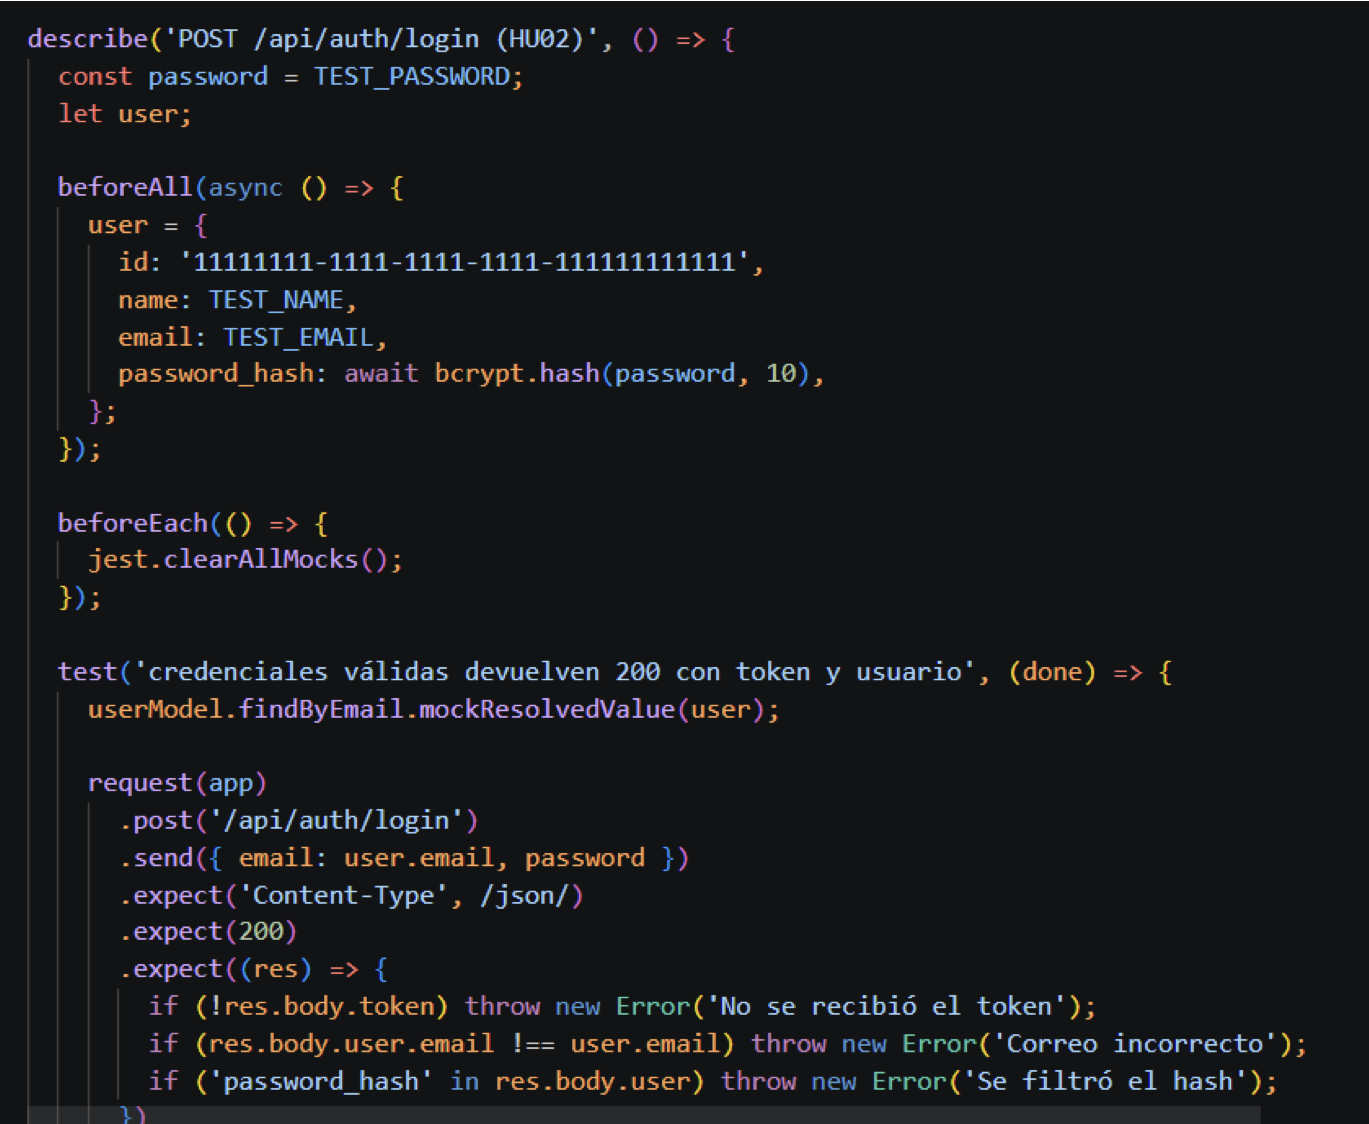
\includegraphics[width=0.8\textwidth]{fig-4-17-estructura-pruebas}
  \caption[Pruebas Unitarias]{Estructura de pruebas unitarias.}
  \label{fig:estructurapruebas}
\vspace{-5.72pt}
\end{figure}

La Figura \ref{fig:resultadopruebas} muestra los resultado de la ejecución de las pruebas unitarias.

\begin{figure}[h]
  \centering
  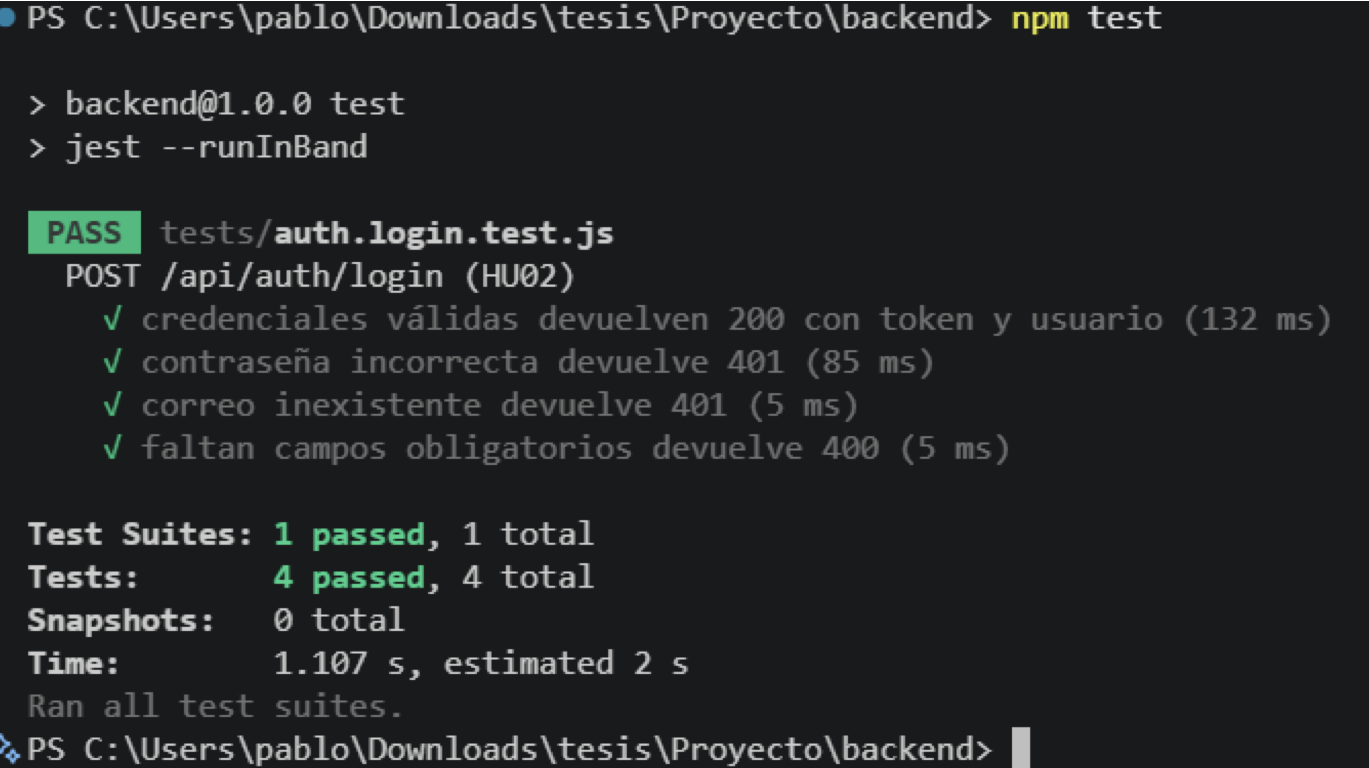
\includegraphics[width=0.8\textwidth]{fig-4-18-resultado-pruebas}
  \caption[Resultado Pruebas Unitarias]{Resultado de la ejecución de pruebas unitarias.}
  \label{fig:resultadopruebas}
\vspace{2.33pt}
\end{figure}

\tituloparpegado{Sistema de pruebas}
Después de la implementación, se lleva a cabo una fase de pruebas para esta iteración, evaluando los siguientes casos:

\begin{itemize}
  \item Ingresar con credenciales válidas.
  \item Ingresar a una ruta que no existe.
  \item Ingresar con un usuario que no existe.
  \item Ingresar con una contraseña incorrecta.
  \item Solicitar recuperación de contraseña con un correo registrado.
  \item Solicitar recuperación de contraseña con un correo no registrado.
  \item Solicitar recuperación de contraseña con un correo con formato inválido.
  \item Solicitar recuperación de contraseña sin ingresar un correo.
  \item Cerrar sesión correctamente.
\end{itemize}

\vspace{\parskip}
\tituloparpegado{Retrospectiva}
Al finalizar la iteración, se revisa si las estimaciones de tiempo para las historias de usuario fueron precisas y se identifican posibles mejoras en el proceso de desarrollo. En este caso, las estimaciones fueron acertadas, y se completaron todas las funcioanlidades planeadas sin pendientes.
